\documentclass[a4paper,11pt]{article}
\pdfoutput=1 % if your are submitting a pdflatex (i.e. if you have
             % images in pdf, png or jpg format)

\usepackage{jinstpub} % for details on the use of the package, please
                     % see the JINST-author-manual


\title{Beam test study of SiPM-on-tile geometries}


%% %simple case: 2 authors, same institution
%% \author{A. Uthor}
%% \author{and A. Nother Author}
%% \affiliation{Institution,\\Address, Country}

% more complex case: 4 authors, 3 institutions, 2 footnotes
%\author[a,b,1]{F. Irst,\note{Corresponding author.}}
%\author[c]{S. Econd,}
%\author[a,2]{T. Hird\note{Also at Some University.}}
%\author[c,2]{and Fourth}

% The "\note" macro will give a warning: "Ignoring empty anchor..."
% you can safely ignore it.

%\affiliation[a]{One University,\\some-street, Country}
%\affiliation[b]{Another University,\\different-address, Country}
%\affiliation[c]{A School for Advanced Studies,\\some-location, Country}

% e-mail addresses: only for the forresponding author
%\emailAdd{first@one.univ}




\abstract{Abstract...}



\keywords{Only keywords from JINST's keywords list please}


\arxivnumber{1234.56789} % only if you have one


% \collaboration{\includegraphics[height=17mm]{example-image}\\[6pt]
%   XXX collaboration}
% or
%\collaboration[c]{on behalf of the XXX collaboration}


% if you write for a special issue this may be useful
%\proceeding{N$^{\text{th}}$ Workshop on X\\
%  when\\
%  where}



\begin{document}
\maketitle
\flushbottom

\section{Introduction}
\label{sec:intro}

The High Luminosity phase of the Large Hadron Collidor (HL-LHC)~\cite{a} is scheduled to begin at CERN in 2027 and it is planned to level the instantaneous luminosity at $5\times 10^{34}\text{cm}^{-2}\text{s}^{-1}$. In order to properly handle this environment, a new high granularity calorimeter (HGCAL)~\cite{b} will be installed in the endcap regions of the CMS detector.

We report the responses of a variety of scintillator tile geometries tested using the Fermilab Testbeam Facility (FTBF) at the Fermi National Accelerator Laboratory.

\section{Testbeam setup}
\label{sec:setup}
\section{DAQ setup}

The Fermilab Testbeam Facility (FTBF) provides a primary beam containing 120 GeV protons bunched at 53 MHz. The beam is delivered as a slow spill with a 4.2 second duration once per minute and an intensity of approximately $5\times10^{4}$ protons per spill. The beam spot size is roughly 4 cm with a sigma in x and y of about 1.5cm, to provide an reasonably even population of protons across our scintillator tiles. 

Describe the scintillator teststand setup...

To provide tracking information, on either side of the black box were planes of silicon pixels with a total square active area of $3.8\times3.8 \mathrm{cm}^{2}$. Get details on the pixel sizes and ROCs from Lorenzo.





\section{Simulation}
\label{sec:simu}

The responses of various tile geometries are estimated with Monte-Carlo simulation based on the Geant4 toolkit\cite{geant4}.
The expected light yield is compared with real data in section xx.

%simulation geometry
Figure \ref{fig:g4simu}. is a schematic drawing describing simulation geometry. 
The SiPM-on-tile geometry can be seperated into two parts, 
one is the tile with a dimple and the other is the SiPM on the backplate. 

The tile is square and enveloped in a thin wrapping layer which helps to increase the light collection.
In center of the tile, a spherical dimple is dug out to make space for SiPM.
A hole is also placed on the wrapping behind dimple so that SiPM could pass through.

SiPM geometry follows from the realistic size in scintillator test.
Behind SiPM is a layer of backplate, which is slightly larger than the hole to prevent photons from escaping.
All in all, we are tying to mimic the testbeam setup. 

%this graph should be changed later
\begin{figure}[htbp]
\centering % \begin{center}/\end{center} takes some additional vertical space
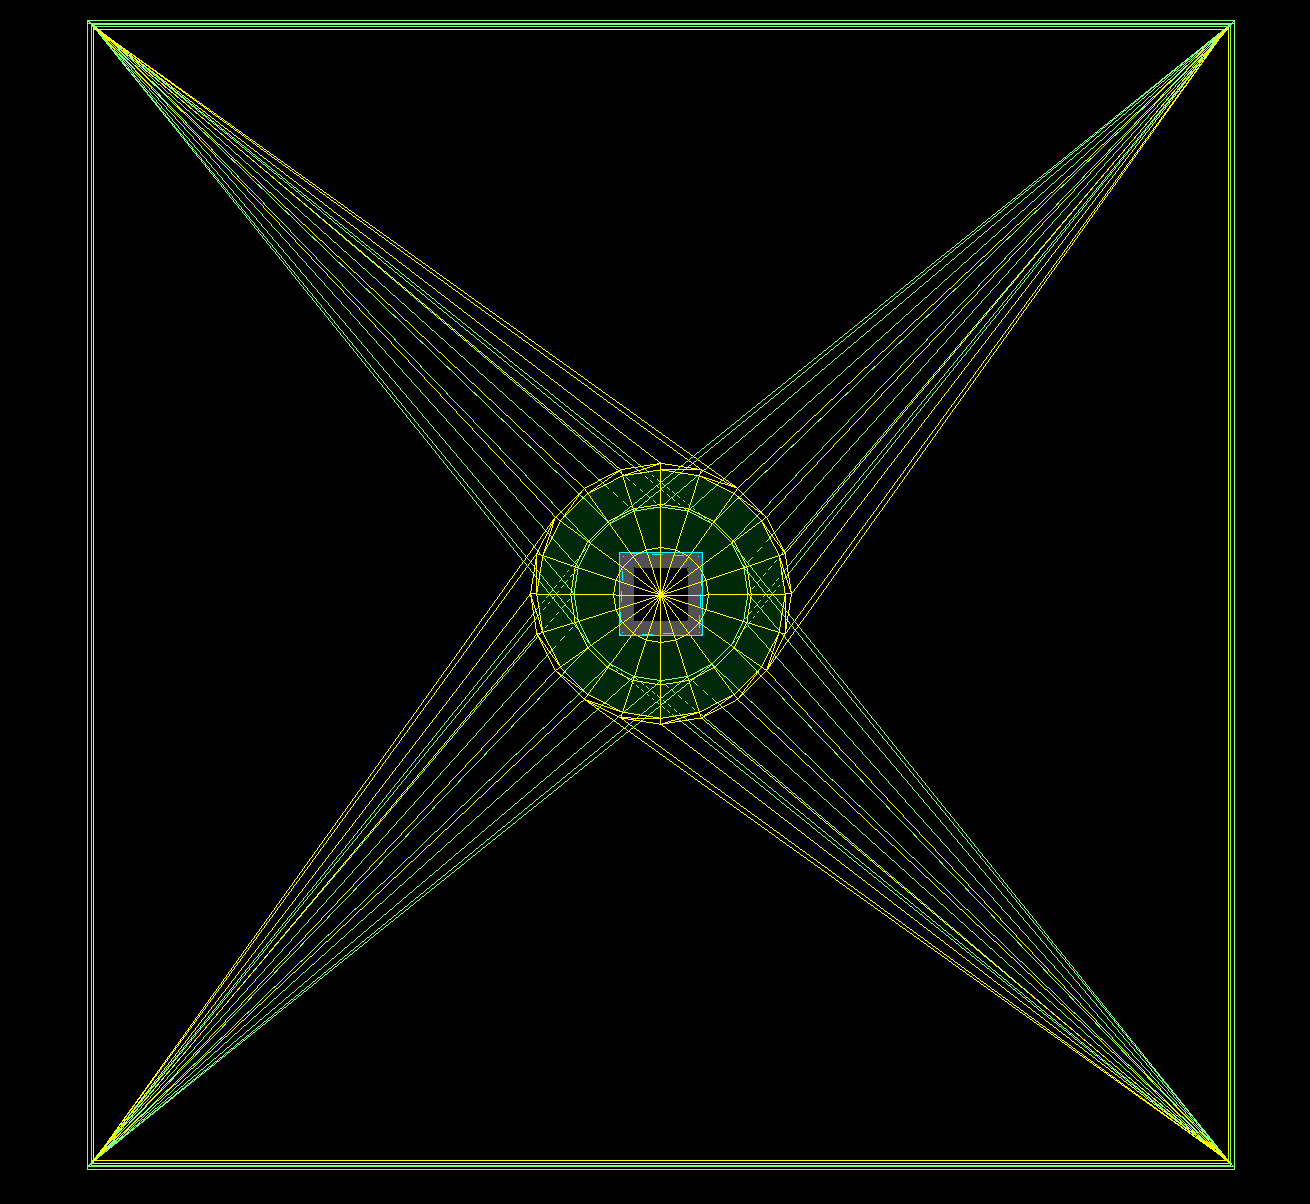
\includegraphics[width=.45\textwidth]{front.png}
%\qquad
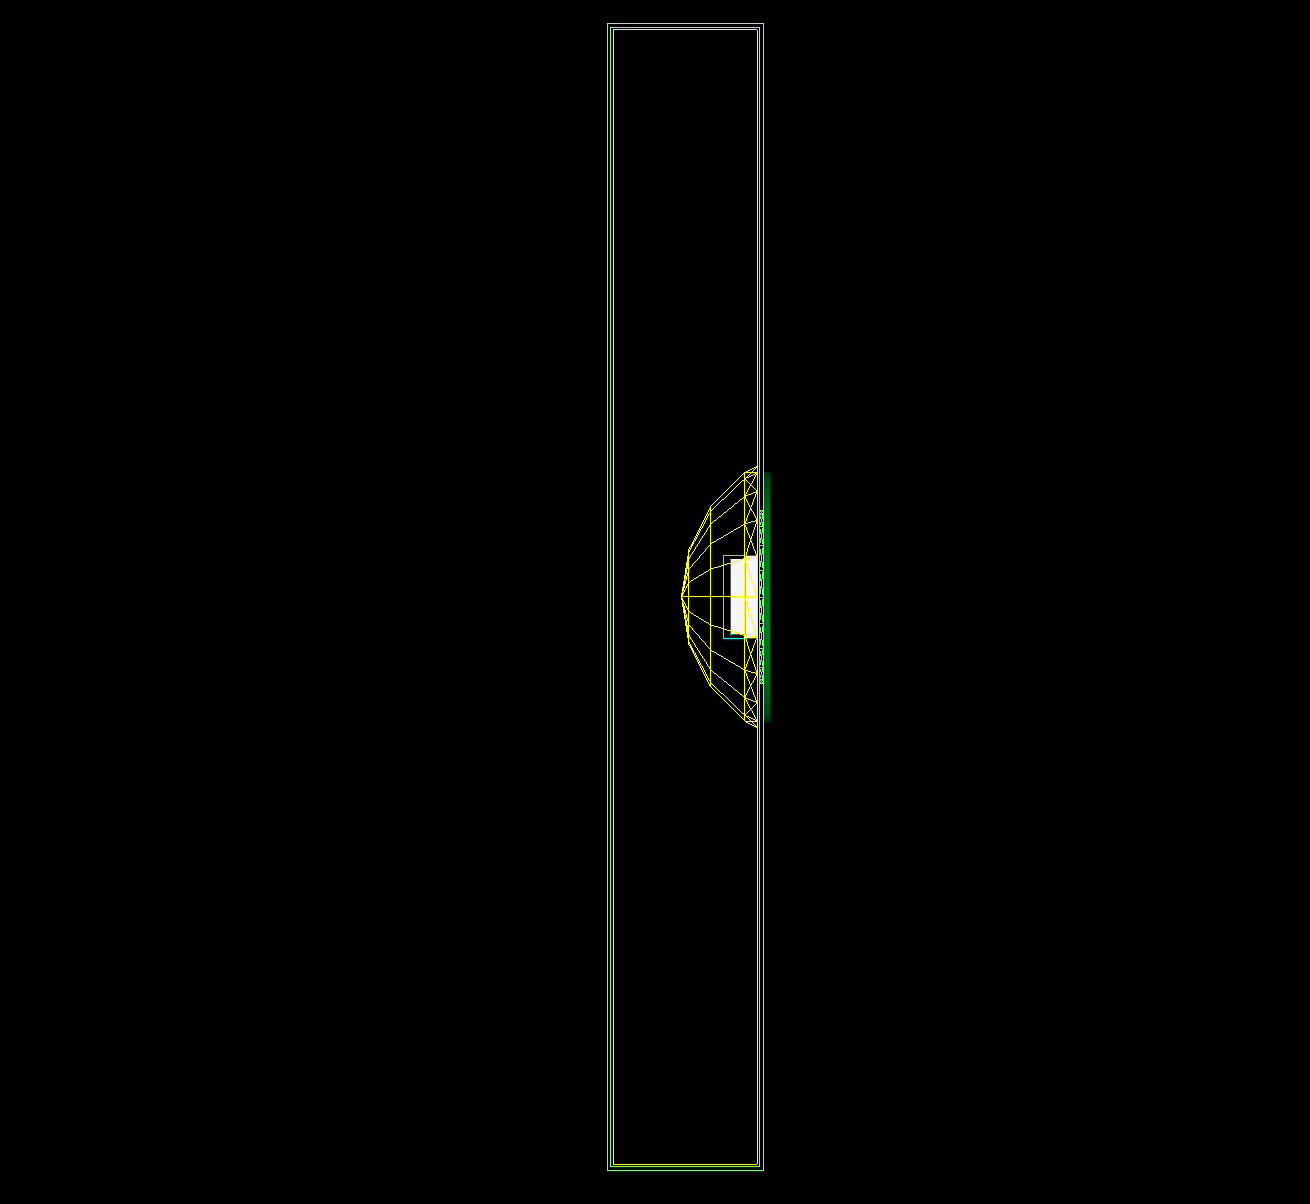
\includegraphics[width=.45\textwidth]{side.png}
% "\includegraphics" from the "graphicx" permits to crop (trim+clip)
% and rotate (angle) and image (and much more)
\caption{\label{fig:g4simu} Simulation geometry}
\end{figure}

%Physics simulation
To speed up the simulation, we start directly from scintillation photons rather than the 120 GeV protons.
The mean number of photons is proportional to the thickness of scintillator that protons have traveled, 
as shown in equation \ref{eqn:nphotons}. 
\begin{equation}
\label{eqn:nphotons}
    N_{\gamma}=\frac{d E}{d x} \cdot \varepsilon \cdot L
\end{equation}
$N_{\gamma}$ is the mean number of generated photons.
$\frac{d E}{d x}$ is the rate of energy loss \cite{pdgdata}.
$\varepsilon$ is the scintillating efficiency \cite{scinti_eff}.
$L$ is the thickness of traveled scintillator.

%Not sure if I need to put reasons here
%There are several reasons why we think such a skip is acceptable. 
%First of all, we care more about the detection efficiency of photons than the exact number. 
%Thus, in our simulations, factors like the reflectivity of wrapping, tile and dimple sizes are more worthwhile to investigate.
%Secondly, the thickness of tile is of 3, 3.8 millimeters. 
%Energetic protons could penetrate the tile easily and the path is more or less a straight line.
%The number of photons is propotional to the energy deposition and photons are uniformly generated inside scintillator. 

In each single simulation, 
the exact number of photons is calculated through Possion distribution with mean of $N_{\gamma}$.
The scintillation process is mimicked by generating photons randomly along the expected proton path. 
Indeed, our simulation is used to estimate how many photons could finally reach the SiPM.
The photon emmission spectrum, photon absorption length of the tile and SiPM quantum efficiency are 3 wavelength dependent optical properties in simulation,
while the reflective properties are wavelength independent.

%more details on the simulation
We systematically studied the scintillator response 
by changing tile cross sectional area, tile thickness and tile hole size.
For each geometry, the proton beam spot is uniformly chosen across tile face and simulation is repeated many times.
The average of detected photons is calculated to represent the expected response of this geometry.
%currently the uncertainty is the standard error, but the processing of simu data should stay the same as the real data. May be changed later.
The results are shown in section xx and compared with test beam data.






\section{SiPM calibration}
\label{sec:calibration}

\section{Simulation Normalization}

\section{Scintillator response}
\subsection{cuts and LY determination ....}
\subsection{Tile uniformity}
\subsection{Tile cross sectional area}

\subsection{Tile thickness}

\subsection{Tile hole size}

\section{Summary}


\begin{thebibliography}{99}

\bibitem{a}
Apollinari G. et al., \emph{High-Luminosity Large Hadron Collider (HL-LHC): Technical Design Report V. 0.1}, CERN-2017-007-M (2017), doi:10.23731/CYRM-2017-004.

\bibitem{b}
CMS Collaboration, \emph{The Phase-2 Upgrade of the CMS Endcap Calorimeter}, CERN-LHCC-2017-023, CMS-TDR-019 (2019), https://cds.cern.ch/record/2293646.

\bibitem{geant4}
S. Agostinelli et al (GEANT4), Nucl. Instrum. Meth. A, 506: 250 (2003)

\bibitem{pdgdata}
http://pdg.lbl.gov/2018/AtomicNuclearProperties/HTML/polyvinyltoluene.html

\bibitem{scinti_eff}
https://eljentechnology.com/products/plastic-scintillators/ej-200-ej-204-ej-208-ej-212

\end{thebibliography}
\end{document}
